\section{Analytical discussion of vertically isothermal disks} 
We begin with a discussion of vertically isothermal disks
where $\Gamma=1$, then $c_s$ is a constant in the shearing box. We
examine separately the limiting case of isothermal perturbations
($\gamma\equiv1$ and any value of $t_c$), nearly-isothermal
perturbations ($\gamma\geq 1$ and $t_c\to0$), and 
adiabatic perturbations ($\gamma\neq 1$ and $t_c\to\infty$).   
\subsection{Isothermal perturbations}\label{iso_discuss}
The linear problem simplifies considerably for the case
$\Gamma=\gamma=1$.  Then 
\begin{align}
  Q=W. 
\end{align}
Inserting this into Eq. \ref{ode_w} gives a single equation for the linear stability
problem for isothermal perturbations in a vertically isothermal disk, 
\begin{align}\label{iso_ode}
  \frac{d^2W}{dz^2} + \left(\frac{d\ln{\rho}}{dz} - \frac{\ii k_x
      r}{D}\frac{d\Omega^2}{dz}\right) \frac{dW}{dz} +
  \sigma^2\left(\frac{1}{c_s^2} + \frac{k_x^2}{D}\right)W=0, 
\end{align} 
subject to appropriate boundary conditions. Eq. \ref{iso_ode} also
applies to $\gamma>1$ for $t_c\to0$. 

We remark that Eq.\ref{iso_ode} is also applicable for    
$\gamma=\Gamma\neq 1$ in the limit $t_c\to\infty$ (i.e. neutrally
stratified adiabatic disks), since in that case  
$Q\simeq W$ as well. However, the following discussion is only
valid for $\gamma=\Gamma=1$ because $c_s$ is taken to be a constant.   

\subsubsection{Approximations}
To facilitate an analytical discussion, we simplify the governing
equation Eq. \ref{iso_ode} with the following approximations:

\begin{enumerate}
\item We consider eigenvalues such that
  $|\sigma^2|\ll \kappa^2$. Then we can replace $D=\kappa^2 -\sigma^2\to
  \kappa^2$. The problem simplifies because the eigenvalue now only
  appears in the last term in Eq. \ref{iso_ode}. We call this the
  low-frequency approximation. 
\item We are mainly interested in the effect of vertical shear, i.e. $q\neq
  0$. This is already captured explicitly in Eq. \ref{iso_ode} through
  the factor $d\Omega^2/dz$. We therefore simplify further by ignoring
  the vertical dependence of $\kappa^2$ elsewhere. For clarity, we
  will replace $\kappa^2$ with $\Omega_k^2$. 
  % , although the discussion
  % is unchanged if we replaced 
  % $\kappa^2$ with $\kappa^2(0)$, for example.    
\end{enumerate}
Making both of these approximations is equivalent to the replacement
$D\to\Omega_k^2$.  We will consider sound-speed profiles with $q<0$ in the global 
disk. Then $\Omega^2(z)$ decreases away from the midplane,
and may reach small values for sufficiently large $|z|$, which
invalidates the low-frequency approximation. In principle, then, the
above approximations implicitly limits us to consider thin disks ($\epsilon
\ll 1$) with vertical domain sizes not too large, so that the rotation
is nearly-Keplerian.   


\subsubsection{Neccessity of vertical shear for
  instability}\label{integral_relation} 
With the above approximations and introducing the dimensionless variables
\begin{align}
  \hat{z} = z/\Hiso,\quad \hat{k}=k_x\Hiso, \quad \hat{\sigma} = \sigma/\Omega_k,
\end{align}
the governing equation can be re-written as
\begin{align}
  0 = W^{\prime\prime} + \left[\ln\rho^\prime - \ii \epsilon q \hat{k}
    f(\zhat)\right]W^\prime + \hat{\sigma}^2\left(1+\hat{k}^2\right)W,\label{iso_ode1}
\end{align}
where the primes denote $d/d\zhat$ and $f(\zhat)$ is defined such that
\begin{align}\label{fz_shear}
  \frac{d\Omega^2}{d\hat{z}} = \epsilon^2q f(\hat{z})\Omega_k^2.
\end{align}

We can establish a necessary condition for instability by multipling
Eq. \ref{iso_ode1} by $\rho W^*$ and integrate vertically from
$\zhat=\zhat_1$ to $z=\zhat_2$. We neglect boundary 
terms when integrating by parts, by assuming $W$ or
$W^\prime$ vanishes at the boundaries, or that the boundaries are 
sufficiently far away so that the boundary terms are negligible because of the
decaying background density with increasing height. Then,
\begin{align}
  &\hat{\sigma}^2\left(1+\hat{k}^2\right)\int_{\zhat_1}^{\zhat_2}\rho|W|^2d\zhat \notag\\
  &=\int_{\zhat_1}^{\zhat_2}\rho|W^\prime|^2d\zhat 
  +\ii \epsilon q \hat{k}\int_{\zhat_1}^{\zhat_2}\rho f(\zhat) W^*W^\prime d\zhat.\label{integral_relation1}
\end{align}
It follows that for instability ($\imag\hat{\sigma}>0$), it is neccessary to
have $q\neq0$ or more generally $d\Omega^2/dz\neq 0$, i.e. vertical shear.  


\subsubsection{Maximum growth rate}   
Here we show that the growth rate is limited by the maximum vertical
shear in the domain. Writing $\hat{\sigma} = \hat{\omega} +
\ii\hat{\nu}$ with real $\hat{\omega}$ and $\hat{\nu}$, the real and
imaginary parts of 
Eq. \ref{integral_relation1} are
\begin{align}
  &\left(\hat{\omega}^2-\hat{\nu}^2\right)\left(1+\hat{k}^2\right)
  \int_{\zhat_1}^{\zhat_2}\rho|W|^2d\hat{z} -
  \int_{\zhat_1}^{\zhat_2}\rho|W^\prime|^2d\hat{z}
  \notag\\
  &=\real\left[\ii
    \epsilon\hat{k}q \int_{\zhat_1}^{\zhat_2}\rho
    f(\hat{z}) W^*W^\prime d\zhat\right], \notag\\
  & 2\hat{\omega}\hat{\nu}\left(1+\hat{k}^2\right)
  \int_{\zhat_1}^{\zhat_2}\rho|W|^2d\hat{z}\notag\\
  &=\imag\left[\ii
    \epsilon\hat{k}q \int_{\zhat_1}^{\zhat_2}\rho
    f(\hat{z}) W^*W^\prime d\hat{z}\right].
\end{align}
Adding the square of these equations give
\begin{align}
  &\left[|\hat{\sigma}|^2\left(1+\hat{k}^2\right)
    \int_{\zhat_1}^{\zhat_2}\rho|W|^2d\hat{z} -
    \int_{\zhat_1}^{\zhat_2}\rho\left|W^\prime \right|^2d\hat{z}\right]^2\notag\\
  &+4\hat{\nu}^2\left(1+\hat{k}^2\right) 
  \int_{\zhat_1}^{\zhat_2}\rho
  |W|^2d\hat{z}\int_{\zhat_1}^{\zhat_2}\rho\left|W^\prime \right|^2d\hat{z}\notag\\
  &=\left|\ii
    \epsilon\hat{k}q\int_{\zhat_1}^{\zhat_2}\rho
    f(\hat{z}) W^*W^\prime d\hat{z}\right|^2.
\end{align}
It is clear that
\begin{align}\label{sigma_finite_domain} 
  &4\hat{\nu}^2\left(1+\hat{k}^2\right) 
  \int_{\zhat_1}^{\zhat_2}\rho
  |W|^2d\hat{z}\int_{\zhat_1}^{\zhat_2}\rho\left|W^\prime \right|^2d\hat{z}\notag\\
  &\leq\left|
    \epsilon\hat{k}q\int_{\zhat_1}^{\zhat_2}\rho
    f(\hat{z}) W^*W^\prime d\hat{z}\right|^2.
\end{align}
On the left hand side of this inequality, we apply the Cauchy-Schwarz
inequality to obtain
\begin{align}
  &\left( \int_{\zhat_1}^{\zhat_2}\rho
    |W|\left|W^\prime \right|d\hat{z}\right)^2\leq
  \int_{\zhat_1}^{\zhat_2}\rho 
  |W|^2d\hat{z}\int_{\zhat_1}^{\zhat_2}\rho\left|W^\prime \right|^2d\hat{z}.
\end{align}
On the right hand side of Eq. \ref{sigma_finite_domain} we have
\begin{align}
  \left|\int_{\zhat_1}^{\zhat_2}\rho
    f(\hat{z}) W^*W^\prime d\hat{z}\right|\leq \int_{\zhat_1}^{\zhat_2}\rho
  \left|f(\hat{z})W^*W^\prime \right|d\hat{z} \notag\\
  \leq
  \mathrm{max}\left(|f|\right)\int_{\zhat_1}^{\zhat_2}\rho
  |W|\left|W^\prime \right|d\hat{z},
\end{align}
where $\mathrm{max}(|f|)$ is the maximum value of $|f|$ in
$\zhat\in[\zhat_1,\zhat_2]$. Inserting these inequalities into
Eq. \ref{sigma_finite_domain} gives
\begin{align}\label{max_growth}
  |\hat{\nu}|\leq
  \frac{\epsilon |\hat{k} q|}{2\sqrt{1+\hat{k}^2}}\mathrm{max}(|f|). 
\end{align}
Recalling that $f$ represents vertical shear (Eq. \ref{fz_shear}), it
follows that the maximum possible growth rate of unstable modes,
satisfying the above boundary conditions, is limited by the maximum
value of the vertical shear in the domain considered. 

For the vertically isothermal disk we have $|f(\hat{z})| =
|\hat{z}|\left(1+\epsilon^2\hat{z}^2\right)^{-3/2}$, which maximises
at $|\zhat|=1/\sqrt{2}\epsilon$. For vertical domains smaller 
than this height, the growth rate is limited by $|f|$ at the vertical
boundaries considered. For $|\epsilon\hat{z}|\ll1$ we have $f\simeq
\hat{z}$, in which case we can expect growth rates to increase linearly
with the vertical domain size.   %no faster than linear 



\subsubsection{Thin-disk limit}
We can make further progress for thin disks ($\epsilon\ll1$), 
by expanding the background density and vertical shear profile in powers
of $z/r$. To lowest order we obtain 
\begin{align}
  &\frac{\rho}{\rho_0} \simeq 
  \exp{\left(-\frac{\hat{z}^2}{2}\right)} \equiv w(\hat{z}),\label{thin_dens}\\
  &\frac{d\Omega^2}{d\hat{z}} \simeq \epsilon^2q\Omega_k^2\hat{z}, \label{thin_vshear}
\end{align} 
%With this approximation and those in \S\ref{integral_relation}, 
and the governing equation becomes 
\begin{align}\label{iso_ode3}
  W^{\prime\prime} - \left(1 + \ii q\epsilon
    \hat{k}\right)\hat{z}W^\prime  +
  \hat{\sigma}^2\left(1+\hat{k}^2\right)W = 
  0.
\end{align}
We remark that for large $|\hat{k}|$, Eq. \ref{iso_ode3} is the same as
that derived by \cite{nelson13}, although we have taken a different
route.  

To complete the problem we must specify boundary conditions. The 
maximum vertical domain size should be limited by the thin
disk and low-frequency approximations (i.e. $z\lesssim r$).     
It is, however, common to take $\mathrm{max}|z|\to\infty$ and impose
that the kinetic  energy remain bounded at infinity. This 
is appropriate for the density field because both the true density profile 
and its thin-disk approximation decay rapidly away from the midplane.   

However, the thin-disk representation of vertical shear diverges with 
$\hat{z}$, unlike the true vertical shear profile which eventually
decays.  Thus, taking $\zhat_{1,2}\to \pm\infty$ will permit unphysically large growth
rates (as demonstrated below). Nevertheless, the infinite disk is
useful to consider since it permits an analytical discussion. 

\subsubsection{Stability in the absence of vertical shear}
When $q=0$, Eq. \ref{iso_ode3} is
\begin{align}\label{hermite_ode}
  \left[w(\hat{z})W^\prime \right]^\prime + nW
  w(\hat{z}) =0, 
\end{align}
where we have defined a new eigenvalue
\begin{align}
  n \equiv \hat{\sigma}^2(1+\hat{k}^2). 
\end{align} 
Eq. \ref{iso_ode3} is Hermite's differential equation. If we impose
that the kinetic energy density remain bounded at infinity, then  
\begin{align}
  W \propto \He_n(\hat{z}),
\end{align}
and $n$ is a non-negative integer. This translates to a real
eigenfrequency $\sigma$ such that
\begin{align}
  \left|\hat{\sigma}\right| = \sqrt{n}
  \left(1+\hat{k}^2\right)^{-1/2}. 
\end{align}
Since we have assumed $|\sigma^2|\ll \kappa^2\sim \Omega_k^2$, our
analysis is only valid for large wavenumbers such that $\hat{k}^2\gg   
n-1$. Physically, this corresponds to radial length-scales much
smaller than the local disk scale height. 

\subsubsection{Polynomial solutions with vertical shear}\label{iso_poly}
We can seek power-series solution to Eq. \ref{iso_ode3},
\begin{align}
  W(\zhat) = \sum_{l=0}^\infty a_l\zhat^l. 
\end{align}
Then the coefficients must satisfy the recurrence relation
\begin{align}
  (l+2)(l+1)a_{l+2} +
  \left[n - l\left(1+\ii \epsilon q  \hat{k}\right)\right] a_l = 0, 
\end{align}
where $n$ is not neccessarily an integer. Indeed, if we demand
a polynomial of degree $L$ as the solution, then the eigenfrequency
must satisfy
\begin{align}\label{sig2_iso}
\hat{\sigma}^2 = L\left(\frac{1+\ii q \epsilon
    \hat{k}}{1+\hat{k}^2}\right).
\end{align}
The eigenfrequency $\hat{\sigma}$ is therefore complex for
$L\geq1$. We are interested in 
unstable modes for which $\imag{\hat{\sigma}}>0$ is the growth rate and is
given by 
\begin{align}\label{simple_growth}
  \hat{\nu} =\sqrt{
   \frac{L}{2\left(1+\hat{k}^2\right)}\left(\sqrt{1+q^2\epsilon^2\hat{k}^2} - 
    1\right)}. 
\end{align}
For fixed $q$ and $\epsilon$, the growth rate vanishes for both
$\hat{k}^2\to0$ and $\hat{k}^2\to\infty$. The maximum growth rate
occurs at the optimum wavenumber $\hat{k}_\mathrm{opt}$
\begin{align}
  |\hat{k}_\mathrm{opt}| = \sqrt{\frac{2+|\epsilon q|}{|\epsilon q|}},
\end{align}
and
\begin{align}
  \mathrm{max}\left(\hat{\nu}\right) =\frac{\sqrt{L}|\epsilon
    q|}{2\sqrt{1+|\epsilon q|}}. \label{iso_max_growth}
\end{align}
Since $L\geq1$, there is no limit to the maximum growth rate. This is
an artifact of the thin-disk approximation because the vertical 
shear $d\Omega^2/dz\propto z$ increases indefinitely with
height. However, we find Eq. \ref{iso_max_growth} compares well with
numerical solutions of the governing equation for small $L$.      

% This expression can be simplified in the limit $|q|\ll 1$, 
%  \begin{align}\label{simple_growth}
%    \frac{\imag(\sigma)}{\Omega_k} = \pm \sqrt{M} 
%    \frac{q\epsilon\hat{k}}{2\sqrt{1+\hat{k}^2}} \quad\quad (|q|\ll 1), 
%  \end{align}
%  with $M$ being an integer. 

In Appendix \ref{pert_theory} we give an alternative method to
infer instability in the presence of vertical shear without explicitly
solving the governing equation. 

\subsection{Nearly-isothermal perturbations}
The explicit solution developed in \S\ref{iso_poly} is valid for
non-isothermal perturbations $\gamma>1$ if the thermal relaxation
(cooling) timescale $t_c\equiv0$. We may ask how
do the eigenfrequencies and eigenfunctions change when we change
$t_c$ from zero to a small but finite value? For sufficiently small
$t_c$, for which the perturbations may be considered
nearly-isothermal, we expect the new solutions to only differ slighly
from that above. 

% Then we may linearize Eq. \ref{nearly_iso1}---\ref{nearly_iso2} to
% determine the effect of adding small finite cooling. 

We begin by writing the pair of ODEs for $W$ and $Q$
(Eq. \ref{ode_w}---\ref{ode_Q}) in the thin-disk, low-frequency, 
nearly-Keplerian approximations as used previously, as well as
adopting dimensionless co-ordinates and variables, 
\begin{align}
  &\hat{\sigma}^2\left(Q +  \hat{k}^2W\right) \notag\\ 
  &= \hat{z} \left(1 +
    \ii\epsilon q \hat{k} \right)\left[W^\prime - \zhat \left(W -
      Q\right)\right] - \left[W^\prime - \zhat \left(W -
      Q\right)\right]^\prime\label{nearly_iso1},\\
&\beta \hat{\sigma}^2\left(W - \gamma Q\right) + \ii\hat{\sigma}
    \left(W-Q\right)\notag\\
   & = -\beta\zhat\left(\gamma-1\right) \left[W^\prime - \zhat \left(W -
      Q\right)\right]\label{nearly_iso2},
\end{align}
where we recall $\beta = t_c\Omega_k$ is the dimensionless cooling
time. It is evident that for $\beta\equiv 0$, we recover
Eq. \ref{iso_ode3}. 

We linearize Eq. \ref{nearly_iso1}---\ref{nearly_iso2} about a known
solution for $\beta\equiv0$. Let 
\begin{align}\label{nearly_iso_pert}
  \beta \to 0 + \delta\beta,\, W\to W+\delta W,\, Q \to Q+\delta
  Q,\,\hat{\sigma} \to \hat{\sigma} + \delta\hat{\sigma}, 
\end{align} 
where $W=Q$ is the polynomial solution described in \S\ref{iso_poly}
with $\hat{\sigma}^2$ given by Eq. \ref{sig2_iso}. Inserting
Eq. \ref{nearly_iso_pert} into
Eq. \ref{nearly_iso1}---\ref{nearly_iso2} and keeping only first order
terms, we obtain
\begin{align}
  &2\hat{\sigma}\delta\hat{\sigma}\left(1+\hat{k}^2\right)W +
  \hat{\sigma}^2 \left(\delta Q + \hat{k}^2\delta W\right)\notag\\
  &= \zhat \left(1+\ii\epsilon q \hat{k}\right)\left[\delta W^\prime -
    \zhat \left(\delta W - 
      \delta Q\right)\right] - \delta W^{\prime\prime}\notag\\
  &\phantom{=} + \left[\zhat \left(\delta W -
     \delta Q\right)\right]^\prime,\label{nearly_iso3}\\
&\ii\hat{\sigma} \left(\delta W - \delta Q\right) =
\delta\beta\left(\gamma-1\right)\left(\hat{\sigma}^2W - \hat{z}W^\prime\right).\label{nearly_iso4}
\end{align}
This is a pair of inhomogeneous ODEs with a forcing by $W$. The
homogeneous problem is, of course, just the ODE for $\beta=0$ solved
in \S\ref{iso_poly}. Hence we only seek the particular solution. 

We could proceed by considering the entire set of polynomial
solutions for $W$, but it is simplest to look at the fundamental
mode. Thus we consider the `basic state' 
\begin{align*}
  W = \hat{z},\quad \hat{\sigma}^2\left(1+\hat{k}^2\right) = 1 +
  \ii\epsilon q \hat{k},
\end{align*}
then
\begin{align}
  \delta W = b \zhat^3,
\end{align}
where $b$ is a constant to be determined. Eliminating $\delta Q$ from
Eq. \ref{nearly_iso3}---\ref{nearly_iso4}, inserting the above
expressions for $W$ and $\delta W$ and balancing coefficients of
$\zhat$ and $\zhat^3$, we find
\begin{align}
 & 2\left(1+\ii\epsilon q \hat{k}\right) \delta\hat{\sigma} \notag\\& = -6b\hat{\sigma} -
2\ii \delta \beta\left(\gamma-1\right)\left(\hat{\sigma}^2-1\right) - \ii
  \hat{\sigma}^2\delta\beta\left(\gamma-1\right),\\
& 0=  2b\hat{\sigma}+\ii\delta\beta
\left(\gamma-1\right)\left(\hat{\sigma}^2 - 1\right),
\end{align}
where the expression for $\hat{\sigma}^2$ was used. Solving for
$\delta\hat{\sigma}$ gives 
\begin{align}\label{nearly_iso_dsig}
  \delta \hat{\sigma} =
  -\frac{\ii\left(\gamma-1\right)\hat{k}^2\left(\ii\epsilon
    q - \hat{k}\right)^2}{2\left(1+\ii\epsilon q \hat{k}\right)\left(1+\hat{k}^2\right)^2}\delta\beta.
\end{align}
The imaginary part of Eq. \ref{nearly_iso_dsig} is
\begin{align}
   \delta\hat{\nu} =
  -\frac{\left(\gamma-1\right)\hat{k}^2 \left(\hat{k}^2 -
      2\epsilon^2q^2\hat{k}^2 - \epsilon^2q^2\right)}{2\left(1+\epsilon^2 q^2
        \hat{k}^2\right)\left(1+\hat{k}^2\right)^2}\delta\beta.  
\end{align}
Since $\epsilon \ll 1$, introducing finite cooling $\delta\beta>0$
implies $\delta\hat{\nu} < 0$, i.e. stabilization. Interestingly, for both
$\hat{k}\to0$ and $\hat{k}\to\infty$ we find $\delta\hat{\nu}\to0$, so
stabilization by finite cooling is ineffective at very large or very
small scales. We plot Eq. \ref{nearly_iso_dsig} in Fig. \ref{domegadbeta} with
$\epsilon=0.05$, $q=-1.0$ and $\gamma=1.4$. For this disk model the
optimum wavenumber for stabilization is $\hat{k}\sim 5$---$6$.  

% This contrasts to the case without vertical shear
% ($q=0$), in which $\p\hat{\sigma}/\p\beta\to\mathrm{constant}$ as 
% $\hat{k}\to\infty$.  

\begin{figure}
  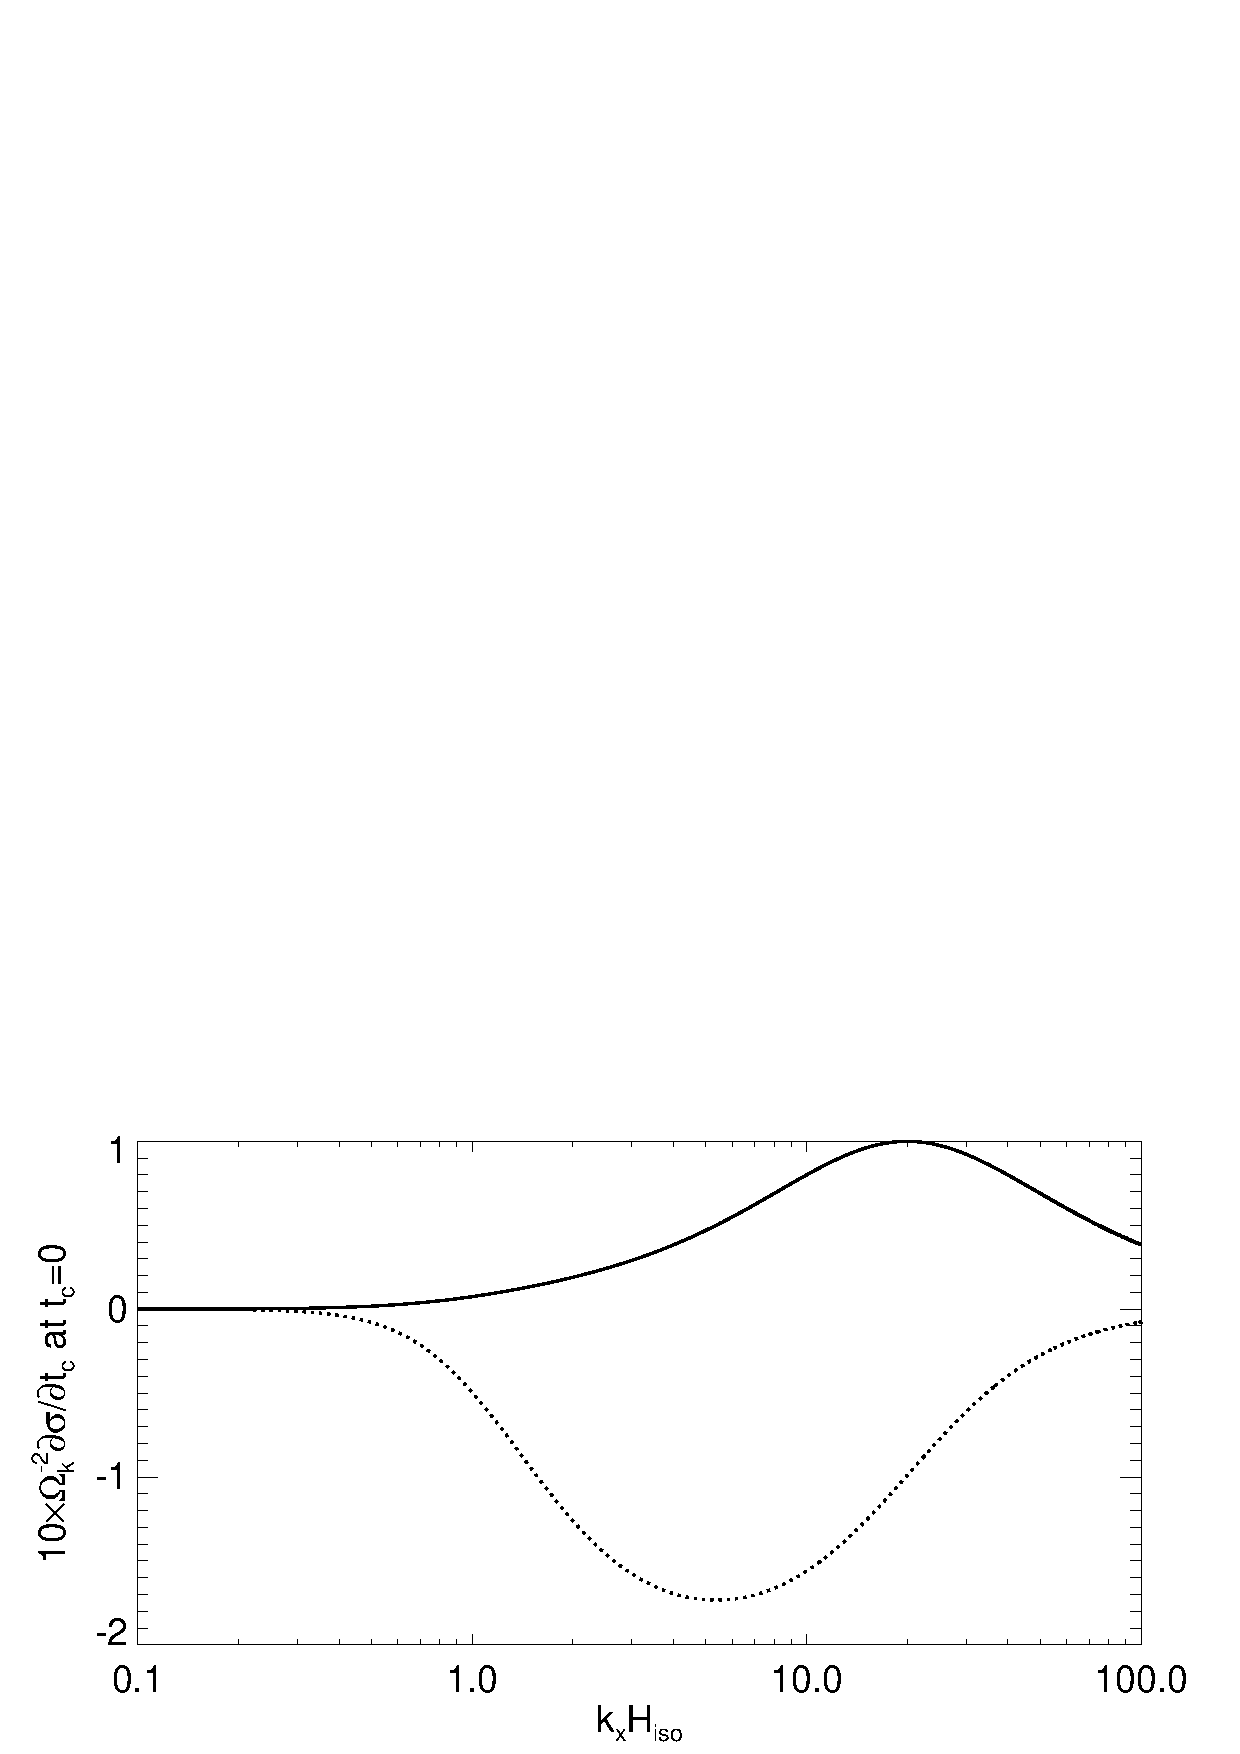
\includegraphics[width=\linewidth]{figures/domegadbeta}
  \caption{Rate of change of the fundamental VSI eigenfrequency
    $\sigma$ with respect to the introduction of a small but finite
    cooling time. The plotted quantity is $\p\hat{\sigma}/\p\beta$ at $\beta=0$, evaluated using
    Eq. \ref{nearly_iso_dsig} with 
    disk parameters $\epsilon=0.05$, $q=-1$ and $\gamma=1.4$. The real
    (imaginary) part of $\p\hat{\sigma}/\p\beta$ is shown as the solid
    (dotted) lines. 
    \label{domegadbeta}}  
\end{figure}   

One effect of introducing finite thermal relaxation is buoyancy. We
show in the next section that buoyancy strongly stabilizes the
VSI. The solution $\delta W\propto\zhat^3$ then makes sense because it
is most significant for large $\zhat$, i.e. away from the midplane
where the effect of bouyancy first appears as $t_c$ is increased. 